%******************************************************************
%******************************************************************
\chapter {Optical Flow Methods}
\label{optical_flow_methods}
%******************************************************************
%******************************************************************

This chapter is dedicated to a detailed description of \opticalflow methods. First we introduce quality measures for motion estimation. Using these measures it is possible to assess the accuracy of the result of the optical flow estimation if the ground truth is known. Then, we present different approaches for the construction of variational models and discuss how these techniques could be applied for X-ray data. This part is divided into several sections, which are devoted to (i) the construction of data constancy assumptions, (ii) robust data terms and (iii) smoothness assumptions. Afterwards we introduce of automated confidence measures.
Next, we extend the devised 2D optical flow models to 3D, which enables us to perform data analysis of tomographic data.  Afterwards, we explain how a variational functional is solved numerically using iterative methods. Furthermore, we discuss various computational aspects such as derivatives discretization and implementation of multi-level computation.


%--------------------------------------------------------
\section{Modeling}
%--------------------------------------------------------

\subsection{Quality Measures}
\label{quality_measures}

Before we start with the description of \opticalflow methods, we first present quality measures which allow for quantitative comparison of different approaches if the ground truth  for \opticalflow is known. We will employ these measures in our extensive performance studies of optical flow methods and data processing techniques in the section \ref{experiments_synthetic_data}. It is important to note, that the performance of an algorithm cannot be described by a single measure. Instead, to show the performance with respect to different characteristics of an image we employ a set of measures. However, we do not show all the available measures for every evaluation. Instead, we use only those measures which are of interest for the particular evaluation case.



\subsubsection{Angular Error}
\label{angular_error}

In the recent years the most widely used performance measure for \opticalflow was the \textit{angular error} (AE). It is given by an angle between a computed flow vector $ \textbf{w} = (u, v)$ and a ground truth flow $\textbf{w}_{GT} = (u_{GT}, v_{GT})$, which can be computed as a dot product of both vectors, divided by the product of their length: 
$$ AE = \text{arccos} \Bigl (\frac{u \cdot u_{GT} + v \cdot v_{GT} + 1.0} {\sqrt{u^2 + v^2 + 1.0} \sqrt{u_{GT}^2 + v_{GT}^2 + 1.0}   } \Bigr ). $$

Note, that angular error contains an additional scaling constant (1.0) to convert from
pixels coordinates to the angular space. This measure was introduced in Ref. \cite{Fleet90} and was used in one of the first surveys on the performance of \opticalflow methods by \cite{Barron94}. The main purpose of the \textit{AE} is to provide a relative performance measure that could be used for all flow scales and is not causing problems for zero motion. However, it is important to note that errors in regions with fast motion are penalized less than errors in slow regions, which is a result of length normalization for this measure. Despite the fact, that the angular error was widely used in the previous work on \opticalflow methods its properties are not desirable for a robust and unbiased measure.


\subsubsection{Endpoint Error}
\label{endpoint_error}

Another measure to estimate the performance of flow field computation is the \textit{endpoint error} (EE) \cite{Otte94}. This measure captures the absolute difference between two flow vectors $\textbf{w} = (u, v)$ and $\textbf{w}_{GT} = (u_{GT}, v_{GT})$:
$$ EE = \sqrt{(u_{GT} - u)^2 + (v_{GT} - v)^2}. $$
The endpoint error does not suffer from the drawbacks of angular error measure: it can be applied for the whole range of flow scales and all of them contribute equally. It is also a much more appropriate way to evaluate the differences between vectors if not only the direction, but also the difference in magnitude of the flow is important. Currently this measure is prevalent in the literature \cite{Sun10, Middl} and will also be used to evaluate the performance of \opticalflow methods in this work. 


\subsubsection{Error Statistics}
\label{error_statistics}

In order to evaluate the result of an \opticalflow computation for a given image sequence one is interested in a quantitative description of the quality of the output. A straightforward statistical measures are the average error  and the standard deviation \cite{Barron94}. Despite the fact, that both measures can be used to evaluate the overall performance, they are not optimal for measuring the performance on challenging image data or more complex scenes (e.g. a scene for which the background with little or no motion is prevalent).

Following the ideas presented in Ref. \cite{Middl} we compute robustness measures \cite{Scharstein02}. For simplicity we also keep their notation for the presented statistical measures and denote by \textit{RX} the percentage of pixels that have an error measure larger then \textit{X}. In particular, we compute \textit{R0.5}, \textit{R1.0}, and \textit{R2.0} for the endpoint error. 

%In addition, we compute robust accuracy measure \cite{Seitz06} for which \textit{AX} denotes the accuracy of the error measure at the X-percentile, after sorting the errors. We report the statistics for \textit{A50}, \textit{A75}, and \textit{A95}.

\subsubsection{Statistics Regions}
\label{statistics_regions}

The reliability of \opticalflow methods differs in various image regions. In particular, it is difficult to compute the flow around motion discontinuities, inside noisy regions, near artifacts or in homogeneous regions. Thus, it is reasonable to distinguish between such regions and evaluate their statistics separately. This can provide insights how different \opticalflow models perform for in a particular situation.  In the common benchmark for \opticalflow methods \cite{Middl} three types of regions were evaluated: all image data (\textit{All}), around motion discontinuities (\textit{Disc}), and in textureless regions (\textit{Untext}). In \cite{Middl} it is concluded that \textit{Disc} regions contain the most challenging data for the computation of optical flow. In contrast, 
textureless regions are not hard to recover, as soon as global optimization techniques (employing smoothness constraints) are used.
In the Section \ref{modeling_xray_data} to evaluate the performance of \opticalflow models on corrupted data we intentionally introduce synthetic artifacts. In this case we are interested to measure error statistics inside these regions and in a local neighborhood around them. We denote such regions with data outliers as \textit{Err} regions.

To compute a mask for the \textit{Disc} regions we take the gradient of
the ground truth displacement field, compute its magnitude, apply a threshold for the magnitude, and then dilate the resulting mask with a $9 \times 9$ stencil. \textit{Untext} regions are computed in a similar manner, but using a $3 \times 3$ stencil size \cite{Middl}. 


%\todo{Consider object and background regions}.



%-------------------------------------
\subsection{Data Constancy Assumptions}
\label{data_constancy_assumptions}
%-------------------------------------


To solve a correspondence problem one has to assume constancy of certain image features. For the choice of an appropriate constancy assumption all prior knowledge about the acquisition method, imaging conditions and the underlying scene should be taken into account. The selection of suitable data  assumptions is essential and should be well adapted for the specific image data. In this section we provide an overview of data constancy assumptions. For each data assumption we discuss the aspects related to its usage on X-ray data.  Note, that in the current work we do not aim to provide a complete list of all data constraints available in the literature. We focus only on those approaches, which can be practically used for highly challenging  X-ray data. For example, we exclude the discussion of data terms based on color information.

\subsubsection{Image Smoothing}
\label{image_smoothing}

The computation of optical flow is usually preceded by a \textit{presmoothing} step. The aim of this step is to eliminate image noise. The most common procedure is to convolve the initial image $I_0$ with a \textit{Gaussian kernel} $K_{\sigma}$ with a standard deviation $\sigma$. High frequency variations are removed due to \textit{low-pass} filtering effect of Gaussian filter.
Furthermore, presmoothed image becomes infinite times differentiable, which is an important property to guarantee \textit{well-posedness} of the inverse problem \cite{HSSW01}. 
%------------------
% Not very useful
%------------------
%An example of the Gaussian filtering of X-ray radiographic image is presented in Figure \ref{fig:2_smooth}.

It is important to note that an appropriate choice of the smoothness degree is a crucial task. On the one hand, image presmoothing allows to improve image data and increase signal-to-noise ratio. On the other hand, oversmoothing destroys small image details and edges, which can lead to an inaccurate \opticalflow estimation. For the description of an optical flow model we always provide the initial smoothness level together with other model parameters.

%\begin{figure*}[ht]
%  \centerline{
%    \mbox{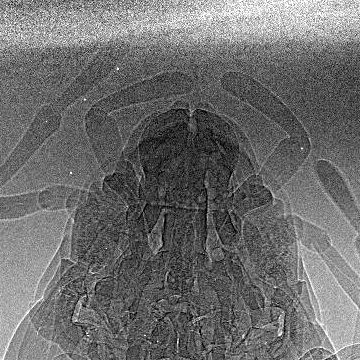
\includegraphics[scale=0.4]{figures/noisy_insect_0p0.png}}
%    \mbox{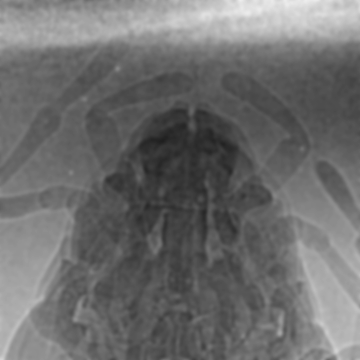
\includegraphics[scale=0.4]{figures/noisy_insect_2p0.png}}
%    \mbox{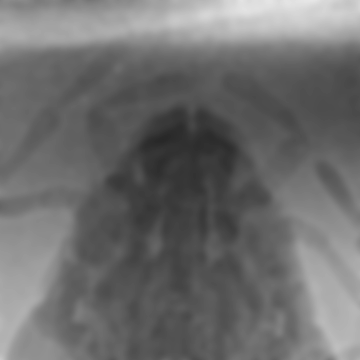
\includegraphics[scale=0.4]{figures/noisy_insect_4p0.png}}
%  }
%  \vspace{3pt}
%  
%  \caption[Performance of Gaussian smoothing]{Performance example of Gaussian smoothing on noisy images of feeding cockroach. Standard deviations $\sigma$ = 0, 2.0 and 4.0 respectively.}
%  \label{fig:2_smooth}
%\end{figure*}



\subsubsection{Brightness Constancy Assumption}
\label{brightness_constancy_assumption}

The simplest assumption is that moving objects within a scene do not change their appearance. In other words, the corresponding pixels have the same brightness values \cite{LucasKanade81, HornSchunck81}. This data constraint combines assumptions about the reflectance properties of the scene and illumination changes. For two subsequent image frames on time $t$ and $t+1$ the brightness constancy assumption can be expressed by:
\begin{equation}
I(x+u, y+v, t+1) = I(x,y,t).
\label{eq:constraint}	
\end{equation}
Under the assumption that the displacement components are small, this non-linear implicit equation for $(u,v)$ can be linearized by performing a first-order Taylor expansion. For a function $I(x+u, y+v, t+1)$ around the point $p = (x, y, t)$ the Taylor expansion is given by:
%------------------
% Not very useful
%------------------
%\begin{figure*}[!h]
%  \centerline{
%    \mbox{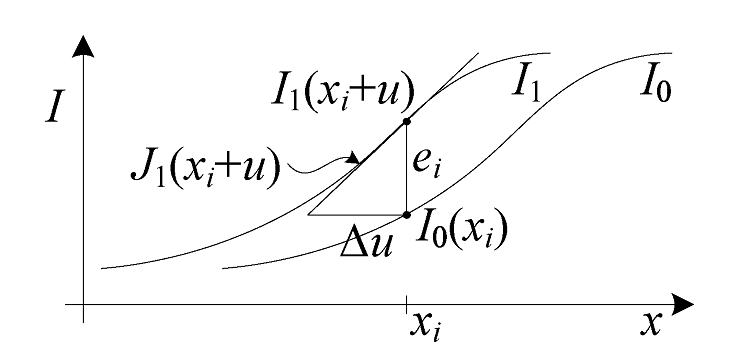
\includegraphics[scale=0.3]{figures/taylor.png}}
%  }
%  \caption[Taylor]{\todo{Correct image} Taylor series approximation of a function $I$ around a point $x_i$ and the incremental computation of the
%optical flow correction amount.}
%  \label{fig:taylor}
%\end{figure*}
$$I(x+u, y+v, t+1) \approx I(x,y,t) + I_{x}u + I_{y}v +I_{t}.$$
Using this approximation, the equation (\ref{eq:constraint}) can be rewritten as:
\begin{equation}
I_{x}u + I_{y}v +I_{t} = 0.
\label{eq:constraint2}	
\end{equation}
which is known in the literature as the \textit{linearized \opticalflow constraint}.

To shorten the formulation of \opticalflow constraints we follow the idea presented in \cite{Bruhn2006} and rewrite the equation (\ref{eq:constraint2}) in the following way:
$$ I_{x}u + I_{y}v +I_{t} = \nabla_{3}^{\top}I\textbf{w}   $$
where $ \textbf{w} = (u, v, 1)$ and $\nabla_{3} = (\partial_{x}, \partial_{y}, \partial_{t})$ denotes the image gradient.

Since both positive and negative deviations from the data constraint should be taken into account, in the work of  \cite{LucasKanade81, HornSchunck81} the authors incorporate its square to the final version of data term. The brightness constancy assumption in a short notation is given by:
$$ D_{grey}(I,\textbf{w}) = (\nabla_{3}^{\top}I\textbf{w})^2.$$



\subsubsection{Gradient Constancy Assumption}
\label{gradient}

The brightness constancy assumption can be used as long as illumination conditions and thus the corresponding pixel grey values between successive frames are not changing. If these assumptions are violated, data constraints that are invariant under brightness changes must be imposed.  To cope with such situations, spatial brightness derivatives are introduced \cite{Uras88, Schnorr93, Brox04, Papenberg06}, since they remain constant in the presence of \textit{additive} illumination.

Taking spatial derivatives of the image brightness for both spatial components we obtain two constraints given by:
$$ I_{x}(x+u, y+v, t+1) = I_{x}(x,y,t), $$
$$ I_{y}(x+u, y+v, t+1) = I_{y}(x,y,t). $$
After linearization step is performed, both constraints using a short notation are given by:
$$ \nabla_{3}^{\top}I_{x}\textbf{w} = 0, $$
$$ \nabla_{3}^{\top}I_{y}\textbf{w} = 0. $$
Combining both constraints gives us the required data term using gradient constancy assumption:
$$ D_{grad}(I,\textbf{w}) = (\nabla_{3}^{\top}I_{x}\textbf{w})^2 + (\nabla_{3}^{\top}I_{y}\textbf{w})^2. $$

It is important to note - that in contrast to the brightness assumption - the gradient assumption provides two independent constraints instead of one. This gives an additional information and could be used to overcome the aperture problem \cite{HornSchunck81}.
However, despite the advantages of gradient assumption in the presence of global brightness changes, this constancy assumption is much more sensitive to noise.
This property of a data constraint is crucial for noisy data, such as often encountered in time-resolved X-ray imaging.  We investigate the influence of noise on the performance of data constancy assumptions in the experimental section \ref{experiment_data_terms_for_noisy_data}.


\subsubsection{High-Order Constancy Assumptions}
\label{high_order_constancy}

The use of derivative-based constancy assumptions is not limited to the constancy of the brightness gradients. Higher-order derivatives, such as the Laplacian could also be employed for formulations of constancy assumptions. However, some of them are not suited for all types of motion. This is due to the fact, that some of these assumptions (e.g. brightness gradient) contain directional information, so they are dependent on the spatial orientation of image features. For an extended taxonomy of possible higher-order constancy assumptions the reader is referred to the literature \cite{Papenberg06}. Here we describe two constraints based on higher-order derivatives which can be potentially useful.
\\
\\
\textbf{Laplacian Constancy Assumption}
\\
As it was mentioned in the previous section, directional information contained in data constraints may introduce some difficulties in the presence of fast rotational motion. To overcome this problem one can restrict to direction-invariant features such as constancy of Laplacian \cite{Papenberg06}, which is given by:
$$ \Delta_{2} I(x+u, y+v, t+1) - \Delta_{2} I(x,y,t) = 0, $$
where $\Delta_{2} I = I_{xx} + I_{yy} $.
The linearized data term in a compact form reads:
$$ D_{lapl}(I,\textbf{w}) = ( \nabla_{3}^{\top}(\Delta_{2}I) \textbf{w})^2.$$

In general, all constraints based on higher-order derivatives are more sensitive to noise and data artifacts than their counterparts based on image intensity. This crucial property must be taken into account for modeling of a suitable energy functional. We compare the performance of the brightness constancy assumption and assumptions based on  derivatives in the evaluation section \ref{experiment_data_terms_for_noisy_data}.
\\
\\
\textbf{Gradient Norm Constancy Assumption}
\\
Another possibility to deal with  fast rotational motion is to use the magnitude of the gradient, instead of spatial gradients themselves (\cite{Papenberg06}).
The obtained data constraint and its corresponding data term are given by:
$$ |\nabla I(x+u, y+v, t+1)| - |\nabla I(x,y,t)| = 0 $$
$$ D_{grad-norm}(I,\textbf{w}) = (\nabla_{3}^{\top}|\nabla I| \textbf{w})^2, $$
where $|\textbf{f}| = \sqrt{f^2_x + f^2_y}$.

\subsubsection{Assumptions on Multiple Image Features}
\label{assumptions_on_multiple_image_features}

To improve the accuracy of \opticalflow computation it might be a good idea to combine assumptions on various image features. The model based on multiple constancy assumptions provides more flexibility and may lead to a significant improvement of the results. An example for this approach a linear combination of both brightness and gradient constancy assumptions \cite{Brox04, HarmonyFlow}. Its data term reads:
$$ D_{brigh+grad}(I,\textbf{w}) = \beta_{1}( \nabla_{3}^{\top}I \textbf{w})^2 + 
\beta_{2} ((\nabla_{3}^{\top}I_{x}\textbf{w})^2 + (\nabla_{3}^{\top}I_{y}\textbf{w})^2), $$
where $\beta_{1}$ and $\beta_{2}$ are parameters to control the contribution of the individual constancy assumption to the overall data term.

Multiple image assumptions might also be useful to incorporate the information obtained by different contrast mechanisms, for example absorption and phase contrast. An alternative approach to include multiple assumptions on image features (and more generally, on different optical flow models) was presented in \cite{Lempitsky08}. In this work a series of candidate flow fields is computed using different algorithms or model parameters. Then a final flow is determined by an additional optimization problem. This idea corresponds to a so-called \textit{fusion} approach. 


\subsubsection{Landmarks-driven approach}
\label{landmarks}


It is possible to incorporate user-defined landmarks to an \opticalflow model. This procedure is especially useful if the manual tracking of some objects or their parts is performed. Thus, it is possible to combine the  information specified by an user with an automated flow computation. As it was shown in \cite{Fischer03} it is not convenient to embed the information about landmarks into the original energy functional. It is much more straightforward to modify the corresponding Euler-Lagrange equations (see Section \ref{minimization_procedure}) directly. We illustrate this on the example of the Horn and Schunck model. 
For this purpose we introduce a confidence map $c_{GT}(x,y)$, which equals to 1 or 0, depending on whether for a pixel position $(x,y)$ the ground truth landmark is given.

Embedding the confidence map $c_{GT}(x,y)$ into the Euler-Lagrange equations (\ref{eq:euler}) we obtain:
$$ (1 - c_{GT}) (I^2_x u + I_x I_y v + I_x I_t - \alpha \: \textrm{div} (\Psi'(|\nabla u|^2 + |\nabla v|^2) \cdot \nabla u )) + c_{GT}(u - u_{GT}) = 0, $$
$$ (1 - c_{GT}) (I_y I_x u + I^2_y v + I_y I_t - \alpha \: \textrm{div} (\Psi'(|\nabla u|^2 + |\nabla v|^2) \cdot \nabla v )) + c_{GT}(v - v_{GT}) = 0. $$
If the ground truth displacement is not provided we obtain the original version of Euler-Lagrange equations.
For the other case the solution is set to the ground truth result $u = u_{GT}, v = v_{GT} $. After the flow field is modified according to information provided by landmarks it is propagated to the neighbouring pixels via the regularization term (see Section \ref{smoothness_assumptions}). Furthermore, to enhance the influence of the ground truth it makes sense to increase the smoothness constraint around locations where the correct flow is given. This could be regarded as an adaptive smoothness approach and can be implemented in a similar way as presented in Section \ref{adaptive_smoothness}. 


%-------------------------------------
\subsection{Robust Data Assumptions}
%-------------------------------------


\subsubsection{Robust Modeling}
\label{robust}


To obtain data constraints which take into account both positive and negative deviations from constancy assumptions in the previous sections we used squared data terms. The effect of such a quadratic, energy-like penalty function can be undesired in the presence of image artifacts or other cases, when constancy assumptions cannot be satisfied.  As a result, such data outliers provide a large contribution to the overall energy functional, decreasing the quality of \opticalflow estimation. To overcome this, it is reasonable to penalize such deviations less strictly using a more robust function. There are a number of different penalty functions available in the literature \cite{Black91, Black96, Sun10, Middl}. The most popular choices are: quadratic function $ \Psi(x) = x^2 $, the Charbonnier penalty $\Psi(x) = \sqrt{x^2 + \epsilon^2} $ \cite{Charbonnier94} and the Lorentzian $\Psi(x) = log (1 + \frac{x^2}{2 \sigma^2}) $ \cite{Black96}, which is a non-convex sub-quadratic penalty function. The comparison between them is presented in Figure \ref{fig:2_penalisers}. An important aspect for the modelling of robust data terms is the convexity of the resulting energy functional.  This property implies that a global minimum solution exists and we may use globally convergent algorithms to search for it. For this reason convex penaliser functions are preferred.

\begin{figure*}[ht]
  \centerline{
    %\includegraphics[scale = 1.0]{2_penalisers.JPG} 
    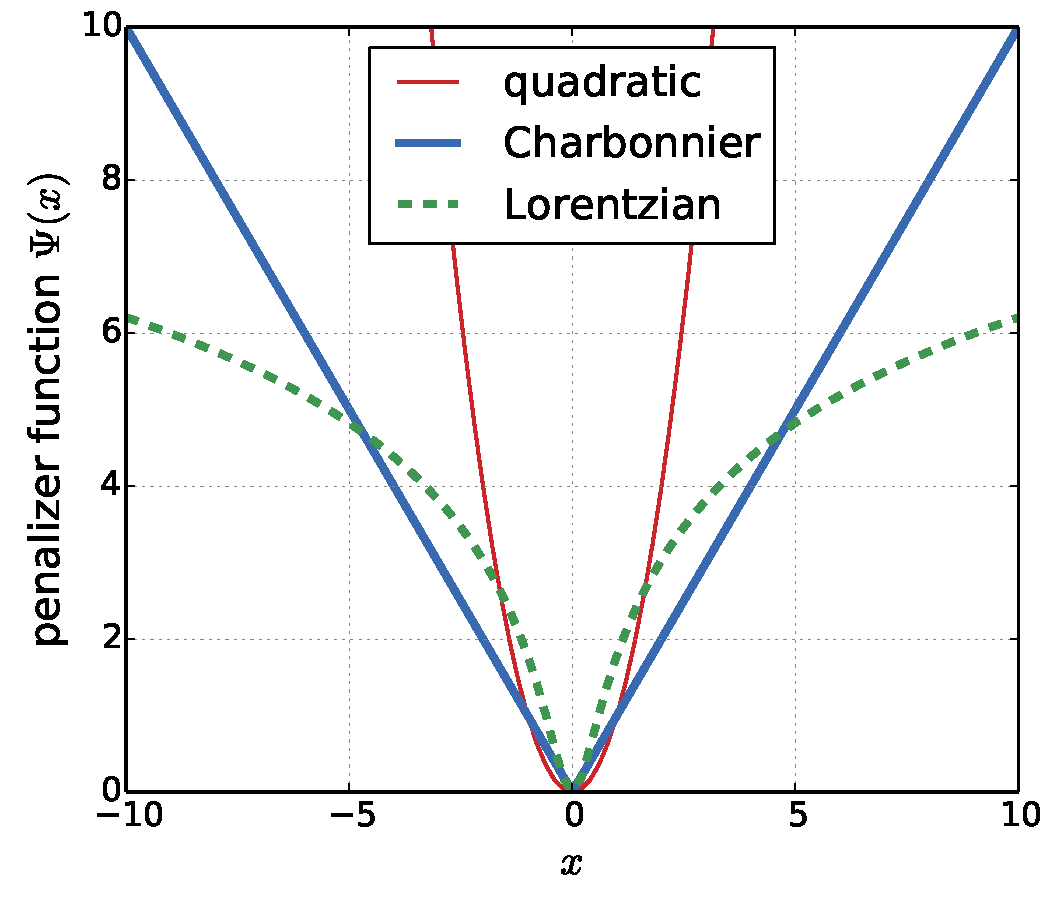
\includegraphics[width=0.45\textwidth]{figures/robust_functions.pdf} 
  }  
  \caption{Comparison between penalising functions: quadratic, Charbonnier and Lorentzian.}
  \label{fig:2_penalisers}
\end{figure*}
For our purpose we choose a penaliser function, which is a differentiable variant of $L_1$-norm \cite{Brox04}:
$$ \Psi_R(x) = \sqrt{x^2 + \epsilon^2},$$
where $\epsilon$ is a small positive constant used to avoid a problem of division by zero after differentiation step.

An example of a robust data term for brightness constancy assumption (see Section \ref{brightness_constancy_assumption}) is given by:
$$ D_{R}(I,\textbf{w}) = \Psi_R ( \nabla_{3}^{\top}I\textbf{w}).$$
As a result of such robust modelling the quality of \opticalflow estimation significantly improves \cite{Sun10, Middl, HarmonyFlow}. We perform quantitative and qualitative evaluation of robust settings in the presence of image artifacts in the experimental sections \ref{experiment_robust_data_term_low_contrast} and \ref{experiment_robust_data_term_low_contrast}.
%\todo{Mention about low contrast here?}

\subsubsection{Joint and Separate Modeling}
\label{joint_and_separate}

In the case when multiple data constraints are used, as we discussed in Section \ref{assumptions_on_multiple_image_features}, an important aspect is how to penalize individual data terms.
One approach is to apply a single penalty function on both data constraints.  On the example of combined brightness and gradient data constancy assumptions this  can be illustrated as:
$$ D_{joint}(I,\textbf{w}) = \Psi_R (\beta_{1}( \nabla_{3}^{\top}I \textbf{w}) + 
\beta_{2} (\nabla_{3}^{\top}I_{x}\textbf{w} + \nabla_{3}^{\top}I_{y}\textbf{w})). $$

Evidently, it is not necessary that both constraints should be satisfied at the same time for all data points. As it was previously shown, brightness constraint fails in regions where illumination changes and gradient constraint is sensitive to noise. However, the deviations from both constraints are penalized jointly. Note, that weight parameters $ \beta_1, \beta_2$ are coupled as an argument of the penalty function, which slightly changes its mathematical formulation. 
 
In the work of \cite{Bruhn05b} the authors introduced a concept of \textit{separate robustification}.
Such strategy takes into account all the data constraints independently and allows to use a different penalty function for each counterpart. Using this approach, we rewrite the combined constraint as:
$$ D_{sep}(I,\textbf{w}) =  \beta_{1}\Psi_{R_1}( \nabla_{3}^{\top}I \textbf{w}) + 
\beta_{2} \Psi_{R_2} (\nabla_{3}^{\top}I_{x}\textbf{w} + \nabla_{3}^{\top}I_{y}\textbf{w}). $$
 
Following the performance analysis from the literature \cite{Bruhn05b, HarmonyFlow}, if multiple image features are used to impose data constancy assumption we choose a separate robustification strategy. Such setting is more flexible and provides better results in most cases.

\subsubsection{Combined Local-Global Approach}
\label{clg}

A useful approach to improve robustness of \opticalflow methods on noisy data is to consider the information not only from a particular data point, but also in a local neighbourhood. The modified data term would then impose a constancy assumption within a fixed region. Such constraint strongly resembles an original \opticalflow method by Lucas and Kanade \cite{LucasKanade81}. In the work of \cite{Bruhn02} so-called \textit{combined local-global} (CLG) approach was introduced. The name highlights the fact that such technique combines the local information for the modelling of data term and provides dense results of global variational methods. 

It is reasonable to weight contributions within a local region according to a distance from the central location (e.g. using weighted least squares fit). In \cite{Bruhn02} it is presented how this approach could be incorporated for the construction of robust data terms. For brightness constancy assumption a least square fit is given by convolution with a Gaussian function: 
$$ D_{CLG}(I,\textbf{w}) =  K_{\rho} \ast (\nabla_{3}^{\top}I\textbf{w})^2, $$
with the standard deviation $\rho$. The standard deviation parameter is also called \textit{integration scale} \cite{Bruhn02}, since it regulates the size of spatial region which is taken into account. 

This approach is not frequently used in the recent works since in cases when a high quality, noise-free data is available it could provide more blurry flow results. However, the combined local-global approach can lead to significant improvements for images which are highly degraded by noise \cite{Bruhn02, Bruhn05a}. We present numerical experiments on noisy data and discuss the usefulness of the local-global approach in the experimental section \ref{experimen_combined_local_global_approach}.


\subsubsection{Normalization of Data Terms}
\label{normalization}

To provide additional robustness in unreliable regions influenced by noise or artifacts it is possible to further adjust the data term.  In the recent work of  \cite{HarmonyFlow} the authors used the ideas presented in \cite{Simoncelli91, Lai98} to perform \textit{normalization} of data constraints. One can show that image locations with large gradient and smooth regions are weighted differently \cite{HarmonyFlow}. As a result, high-gradient features provide more contribution to overall energy of the data term and thus largely influence the estimation of optical flow. Such behaviour can be undesired since high image gradient may be caused by noise or artifacts.
Following \cite{Lai98, HarmonyFlow} the original data constraint can be normalized by a factor:
$$n =  \frac{1}{|\nabla_2 I(x,y,t)|^2 + \eta} , $$
where positive parameter $\eta$ avoids division by zero and controls the normalisation process depending on the noise scale. 

%The influence of normalization is shown in Figure \ref{fig:data_normalization}. 

%\begin{figure*}[ht]
%  \centerline{
%    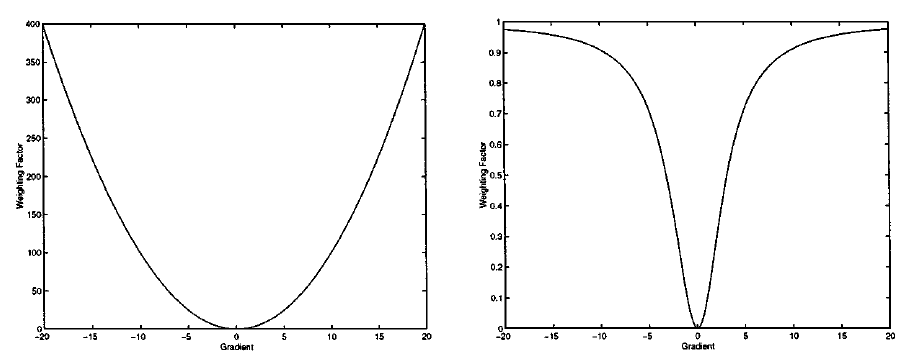
\includegraphics[scale = 0.4]{figures/data_normalization.PNG} 
%  }  
%  \caption{\todo{Remake image}Comparison between the original and normalized data constraint.  \textbf{Left:} Original quadratic weighting. \textbf{Right:} Normalized weighting. }
%  \label{fig:data_normalization}
%\end{figure*}

After the normalization procedure the resulting data term is still convex and can be easily incorporated in our variational computation scheme. The normalized brightness constancy constraint is given by:
$$ D_{norm}(I,\textbf{w}) = n (\nabla_{3}^{\top}I\textbf{w})^2.$$

For low contrast and noisy X-ray images the use of normalized data terms can be especially beneficial. We discuss the influence of proposed correction procedure, as well as choice of the appropriate $\eta$ parameter on various amounts of noise in Section \ref{experiment_normalization_data_term}.

\subsubsection{Refinement Model}
\label{refinement}

In the work of \cite{Xu10} authors proposed to explicitly model occlusions (or other data outliers) and reduce the influence of data term in these regions.  First, a motion estimation is performed using appropriate model assumptions, then a confidence map is constructed using an occlusion detection. Then, a second run of optical flow algorithm is done using occlusion-aware refinement:
$$E_{refine}(I, \textbf{w}) = \int_{\Omega}{(c(\textbf{x}) \cdot \: D(I, \textbf{w}) + \alpha   S(I, \textbf{w})) \: \text{d}\Omega},$$
where $c(\textbf{x})$ is a confidence map, which downweights the contribution of data constraint for unreliable image regions, $D(I,\textbf{w})$ is a data constraint and $S(I, \textbf{w})$ regulates the smoothness properties of the flow field. 

We discuss various approaches for the estimation of confidence maps in Section \ref{confidence_measures}.


%-------------------------------------
\subsection{Smoothness Assumptions}
\label{smoothness_assumptions}
%-------------------------------------


As it was mentioned previously, assuming constancy constraints based only on local image data is not sufficient to uniquely find a solution for optical flow. In order to overcome the aperture problem additional assumptions about the  flow field itself are employed. The first idea to impose such assumptions goes back to the seminal work of Horn and Schunck \cite{HornSchunck81}. Smoothness constraints allow a \textit{filling-in} \cite{Weickert00b} of the flow information from the adjacent regions at image locations where no unique correspondence can be determined. Most of the approaches impose smoothness constraint by penalizing the magnitude of the flow gradient. 
According to the specific properties of the smoothness one may distinguish between \textit{homogeneous}, \textit{isotropic} and \textit{anisotropic} smoothness. For a more detailed description of various models we refer the reader to the work of \cite{Weickert00b}.

\subsubsection{Homogeneous Smoothness}
\label{homogeneous_smoothness}

The original method of Horn and Schunck \cite{HornSchunck81} introduces smoothness assumption by penalizing magnitude of the flow gradient:
$$ S_{HS}(u,v) = u_{x}^2 + u_{y}^2 + v_{x}^2 + v_{y}^2 = |\nabla_2 u|^2 + |\nabla_2 v|^2,$$
where $|\textbf{f}| = \sqrt{f^2_x + f^2_y}$ is a spatial magnitude and $\nabla_2 = (\partial_{x}, \partial_{y})$ denotes a spatial gradient.
This \textit{homogeneous} regularization requires uniformly smooth flow fields and does not adapt to any supplementary information about image data and the flow field. Assuming that depicted objects may move differently from the background or with respect to each other it is evident that such constraint can hardly be fulfilled. Therefore, smoothness assumptions which allow to model discontinuities more thoroughly are required.

\subsubsection{Image-Driven Smoothness}
\label{image_driven}

In order to take into account motion discontinuities one may assume that the flow field coincides with the boundaries of moving object, thus the smoothness degree can be adjusted according to image edges  \cite{Nagel86, Alvarez99}. To implement this approach one can multiply the original smoothness term by a scalar weighting function $g(x)$ that decreases on image edges \cite{Schnorr93, Alvarez99}. One possibility for such function is:
$$ g(x) = \frac{1}{2 \sqrt{x + \epsilon}}, $$
where $\epsilon$ is a small positive constant used to avoid a problem of division by zero.

The obtained \textit{image-driven} smoothness term is given by:
$$ S_{image}(I,u,v) = g(|\nabla I|^2)(|\nabla u|^2 + |\nabla v|^2), $$
where the magnitude of the spatial gradient $|\nabla I|$ is used to identify image edges \cite{Weickert00b}. It should be noted, that such smoothness term is isotropic, since it treats all directions in image gradients in the same manner. To enhance the smoothing process along image edges, and suppress across them one can use an anisotropic image-driven approach \cite{Nagel86}. 

Despite the fact that image-driven regularization provides sharp edges on the boundaries of moving object, it is prone to errors if the image gradient does not correspond to the actual flow discontinuities. For instance, this occurs in highly textured regions. Image noise is another challenge for this method, which causes the smoothness value to be adjusted to noise variations. In both cases image-driven approaches produce oversegmentation artifacts in the computed flow field. 

\subsubsection{Flow-Driven Smoothness}
\label{flow_driven}

To preserve motion discontinuities the smoothness can be adapted to the unknown flow field. In this case the smoothness is reduced at flow edges described by the flow gradient \cite{Shulman89, Schnorr94}.
The regularization based on the \textit{flow-driven} approach is thus given by:
$$ S_{flow}(u,v) = \Psi_{S}(|\nabla u|^2 + |\nabla v|^2), $$
where the smoothness penalty function reads  $\Psi_{S}(x) = \sqrt{x + \epsilon}$ and corresponds to the total variation (TV) regularization \cite{ROF92}.

In comparison to image-driven method the flow-driven approach provides less strict estimation of flow edges on the boundaries of the moving objects. However, for high-texture or noisy data the flow-driven approach is more robust and outperforms image-driven flow regularization \cite{Brox04, Papenberg06, Wedel09}.   



%\subsubsection{Anisotropic Smoothness}
%\label{anisotropic_driven}
%
%\comment{Info from Bruhn thesis}
%
%\change{From: \cite{Middl}. In (10) the weighting function is isotropic, treating all directions equally. A variety of approaches weight the smoothness
%prior anisotropically. For example, Nagel and Enkelmann
%(1986) and Werlberger et al. (2009) weight the direction
%along the image gradient less than the direction orthogonal
%to it, and Sun et al. (2008) learn a Steerable Random
%Field to define the weighting. Zimmer et al. (2009) perform
%a similar anisotropic weighting, but the directions are defined
%by the data constraint rather than the image gradient.}
%
%\change{From: \cite{HarmonyFlow} An anisotropic counterpart that also exploits the
%directional information of image discontinuities was introduced by Nagel and Enkelmann (1986). Their method regularises the flow field along image edges but not across them.
%As noted by Xiao et al. (2006), this comes down to convolving the flow field with an oriented Gaussian where the orientation is adapted to the image edges.}
%
%\change{From: Bruhn. Flow-driven regularisers take into account discontinuities of the unknown flow field u
%by preventing smoothing at or across flow discontinuities. If the resulting diffusion process
%uses a scalar-valued diffusivity that only depends on |ru|2 := |ru1|2 + |ru2|2, it
%is an isotropic process [Sch94b]. Cases where also the direction of ru1 and ru2 matters
%are named anisotropic [WS01a]. Flow-driven regularisers lead to nonlinear diffusion
%processes.}
%
%For more in-depth qualitative and quantitative comparison of isotropic and anisotropic settings we refer the reader to the work of [WS01a] and Bruhn thesis.


\subsubsection{Spatial-Temporal Smoothness}
\label{spatial_temporal}

In case if more then two frames are given for the estimation of optical flow, it is reasonable to additionally assume temporal smoothness of the flow fields \cite{Murray87, Black91}. For variational approaches such spatial-temporal smoothness terms were proposed by \cite{Nagel90} and \cite{Weickert2001b}.
Implementation of the spatial-temporal smoothness term is done by the extension of spatial derivatives to the spatial-temporal dimension:
$$ S_{temp}(u,v) = u_{x}^2 + u_{y}^2 + u_{t}^2+ v_{x}^2 + v_{y}^2 + v_{t}^2 = |\nabla_3 u|^2 + |\nabla_3 v|^2,$$
where $\nabla_3 = (\partial_{x}, \partial_{y}, \partial_{t})$ denotes the spatial-temporal gradient.


The usage of temporal information provides a significant improvement for the estimation of optical flow \cite{Brox04, HarmonyFlow}. In the case when stationary regions are corrupted by noise the temporal regularization helps to smooth noise contributions and correctly estimate zero flows. This property of spatial-temporal smoothness is especially useful if one is interested in separation between moving objects and a static background, i.e. for motion-based segmentation.
For moving objects the applicability of the temporal smoothness depends on the type and magnitude of displacements. In the case of small, linear displacements the extension to the temporal domain will not cause problems since the influence of spatial and temporal smoothness will be approximately equal. However, in the presence of fast motion large discontinuities in a temporal direction may emerge. To appropriately handle them a number of strategies can be used. One way would be to use the coarse-to-fine computation scheme which allows to solve for large displacements. We describe this technique in details in Section \ref{coarse_strategy}. Another option would be to employ discontinuity preserving smoothness terms using robust penalty function presented in Section \ref{flow_driven}. This approach will result into a joint spatial-temporal discontinuity preserving smoothness term:
$$ S_{flow-temp}(u,v) = \Psi_{S}(|\nabla u|^3 + |\nabla v|^3), $$
where $\Psi_{S}(x) = \sqrt{x + \epsilon}$  and  $\nabla_3 = (\partial_{x}, \partial_{y}, \partial_{t})$.

An important aspect for modeling temporal smoothness is a number of time frames used to impose constraints in temporal direction. In the works of \cite{BruhnThesis}, \cite{HarmonyFlow} it was shown that increasing the number of frames significantly improved the results. However, it was also observed that there is an upper limit after which there is no longer an improvement in the result. The usage of both spatial and temporal information about the flow field allows to decrease the optimal value for smoothness parameter, which result in a sharper flow edges. Additionally, it is reasonable to apply presmoothing step described in Section \ref{image_smoothing} also in temporal direction \cite{BruhnThesis}. The temporal smoothness parameter should be chosen according to constancy of the motion in time and amount of noise.
In general, spatial-temporal smoothness provides a robust approach to compute the optical flow, especially for noisy or corrupted data.



\subsubsection{Adaptive Smoothness}
\label{adaptive_smoothness}


The smoothness term can be further adapted using a number of different strategies.
One approach would be to use a weighting function based on segmented masks representing particular data objects. Such objects could be identified during the optical flow computation or can be pre-labeled using an a-priori knowledge. An example of such masks could be a reduction of smoothness weight on the boundary of closely moving objects, which may improve the separation between them. Another example corresponds to the case when the motion in separate regions expected to exhibit different properties.

The adaptive variant of the smoothness term is then given by:
$$ S_{adapt}(I,u,v) = \alpha_{S_{i}}(|\nabla u|^2 + |\nabla v|^2), $$
where $\alpha_{S_{i}}$ represents the smoothness parameter inside or around the segment $S_{i}$.

Another strategy is to adapt the smoothness according to the computation procedure.
In \cite{HarmonyFlow} authors proposed to adjust the smoothness weight on each level of multiscale computation of optical flow. One may note, that on coarser image levels the data term provides less details resulting from smoothing properties of the downscaling procedure. In this case it makes sense to increase the influence of the smoothness term. This can be done by adjusting the flow regularization according to the warping computation level $k$:
$\alpha(k) = \frac{\alpha}{\eta^k},$
where  $\eta$ is a downscaling factor.



\subsubsection{Joint Image and Flow Driven Smoothness}
\label{image_flow_smoothness}


As it was discussed in Sections \ref{image_driven} and \ref{flow_driven} both image- and flow-driven smoothness approaches have their advantages and drawbacks. To improve the performance of optical flow estimation it makes sense to combine the advantages of both methods to obtain precise motion discontinuities and avoid oversegmentation problems in highly textured image regions. 
The first idea which achieves that was presented in \cite{Sun08}. In this work the smoothness direction is adapted to image edges and smoothing amount to the flow gradient. In \cite{HarmonyFlow} the authors presented a more general approach, which they call \textit{complementary smoothness term}.  Such approach regulates the smoothness direction according to the data constraint, which could be different from information given by image gradients. As a result the smoothness is reduced in the direction where data constraint provides useful information and increased in regions where data constraint is vanished.  





%-------------------------------------
\subsection{Measures of Confidence}
\label{confidence_measures}
%-------------------------------------

In Section \ref{quality_measures} we have described measures for quantitative evaluation of \opticalflow algorithms in the case when the ground truth result is known. In this section we discuss measures to check the reliability of optical flow based only on the computed flow field and initial image data. 
     
Until the recent works of \cite{Sun10, HarmonyFlow} only little attention was dedicated to the application of confidence measures for \opticalflow methods.  
These measures can allow us to determine errors in the computed flow fields caused by artifacts. Moreover, we may use these measures to evaluate the quality of the computed result and automatically optimize the model parameters for the \opticalflow computation.  


\subsubsection{Gradient-based Measure}

The first confidence measure for variational \opticalflow methods was presented by \cite{Barron94}.
It was proposed to relate the quality of the flow estimation with the image gradient, since as it was discussed in Section \ref{general_model} the correspondence problem can only be solved if there is enough information provided by the local image gradient. The confidence measure based on image data is thus given by:
$$ C_{gradient}(\textbf{x}) = |\nabla I(\textbf{x})|. $$
Clearly, this measure does not take into account any dynamical information and assumes only local image data. Additionally, this measure is not capable to evaluate global optical flow approaches which use additional smoothness term to overcome the aperture problem. Moreover, the variations in image brightness can be caused by noise or artifacts. These drawbacks make image-based confidence measure not well suited for the evaluation of optical flow estimation.


\subsubsection{Energy-based Measure}
\label{energy_based_measure}

In the work of \cite{Bruhn06, ErshovThesis} the authors presented an intuitive way to evaluate the quality of variational optical flow methods based on energy minimization. 
Since during minimization  procedure such functionals penalize deviations from model assumptions, it is very natural to consider such deviations as a confidence measure. 

For the case of method of Horn and Schunck the energy-based confidence measure for a pixel \textbf{x} reads:
$$ C_{energy}(\textbf{x}) = \frac{1}{(\nabla_{3}^{\top}I(\textbf{x})\textbf{w})^2 + \alpha ( |\nabla_2 u(\textbf{x})|^2 + |\nabla_2 v(\textbf{x})|^2)}. $$

At this point one may consider to evaluate energy contributions from both data and smoothness terms jointly or, alternatively, evaluate only the data term which constitutes the optical flow problem, i.e. correspondence between pixels (see Section \ref{data_constancy_error}).  
In the presence of artifacts or other data outliers the model assumptions are violated, which results in a high values of energy in those regions.  

As it was discussed in \cite{Bruhn06} energy-based confidence measures have a number of advantages: 1) it is based on the same assumptions as the computational model 2) it is general and could be extended or modified for a particular optical flow model 3) it does not require additional parameters.


\subsubsection{Data Constancy Error}
\label{data_constancy_error}

A similar concept to the energy-based confidence measure is a data constancy error, which evaluates only the data constraint. For the case of brightness constancy assumption, the confidence measure for a pixel \textbf{x} reads:

$$ C_{data}(\textbf{x}) = (I(\textbf{x} + \textbf{w}, t+1) - I(\textbf{x}, t)). $$

This measure shares the same set of advantages as the energy-based confidence measure, as it is also directly based on an optical flow model.


\subsubsection{Motion Uniqueness Criteria}
\label{motion_uniqueness_criteria}

Another approach to evaluate the computed flow field is to examine its spatial distribution. 
We assume that if the motion is applied (source image is warped towards the target image) all pixels should still be uniformly distributed \cite{Brown03, ErshovThesis, Xu10}. However, in the presence of data outliers or problems with appearing and disappearing information the flow vectors could point to nearly the same position. Such multiple pixels mapping could indicate a location of unreliable motion estimation. This idea is illustrated in Figure \ref{fig:4_uniqueness}. 

\begin{figure*}[ht]
  \centerline{
    \mbox{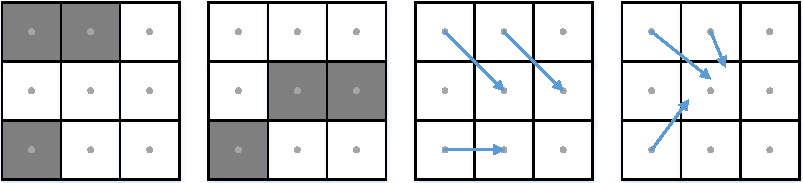
\includegraphics[width=0.9\textwidth]{figures/fig_22_p42.pdf}} 
  }
  \caption[Flow Uniqueness.]{Flow uniqueness criteria. \textbf{Left:} First image frame. \textbf{Middle Left:} Second image frame. \textbf{Middle Right:} One-to-one correspondence. Pixels are mapped to uniformly distributed positions. \textbf{Right:} Pixels are mapped nearly to the same position, indicating a  sink in a vector field.}
  \label{fig:4_uniqueness}
\end{figure*}

In order to implement this approach we count a number of arrived pixels $\textbf{x}+\textbf{u}(\textbf{x})$  to the target image position $\textbf{x}$ . In order to handle real-valued displacements we redistribute contributions from neighboring flow vectors according to their distance to the target pixel location. The confidence measure based on motion uniqueness mapping is then expressed by:
$$ C_{unique}(\textbf{x}) = \frac{1}{|1 - count(\textbf{x})| + \epsilon}, $$
where $\epsilon$ is a small posotive contstant to avoid a division by zero problem.
The deviations from the one-to-one mapping will be captured and the confidence degree will be reduced.


        
\subsubsection{Forward-Backward Check}
\label{forward_backward_check}

A common way to ensure consistency of a motion field solution in the presence of occlusions is to perform a so-called \textit{forward-backward check} (or \textit{cross-checking}) \cite{Chang91, Fua93, Brown03}. In this approach we assume that the flow field computed in forward (from  $I(\textbf{x}, t)$ to $I(\textbf{x}, t+1)$) and the backward direction is equal, but opposite:

%$$ u^{forw}_{ij} = - u^{back}_{i+ u^{forw}_{ij}, j +  v^{forw}_{ij}} $$   
%$$ v^{forw}_{ij} = - v^{back}_{i+ u^{forw}_{ij}, j +  v^{forw}_{ij},} $$
%where $\textbf{w}^{fw}$ and $\textbf{w}^{bw}$ is a flow field computed in forward and backward %direction respectively.

$$ \textbf{w}^{f}(\textbf{x}) = - \textbf{w}^{b}(\textbf{x} + \textbf{w}^{f}(\textbf{x}))$$   
where $\textbf{w}^{f}$ and $\textbf{w}^{b}$ is a flow field computed in a forward and a backward direction respectively.

In the case of occlusions or other image artifacts, forward and backward vectors do not match, which could be exploited to identify problematic regions. For the consistency based confidence measure we estimate the magnitude of the difference vector between forward and backward flow vectors:
$$ |\Delta \textbf{w}(\textbf{x})| = \sqrt { \left ( \textbf{w}^{f}(\textbf{x}) + \textbf{w}^{b}(\textbf{x} + \textbf{w}^{f}(\textbf{x})) \right )^2  }$$

%$$ |\Delta \textbf{w}_{ij}| = \sqrt { \left (u^{forw}_{ij} + u^{back}_{i+ u^{forw}_{ij}, j +  v^{forw}_{ij}} \right )^2 + \left (v^{forw}_{ij} + v^{back}_{i+ u^{forw}_{ij}, j +  v^{forw}_{ij}} \right )^2 }$$

\begin{figure*}[h]
  \centerline{
    \mbox{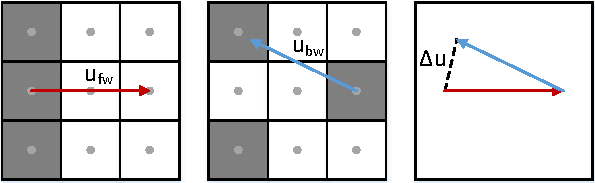
\includegraphics[width=0.7\textwidth]{figures/fig_23_p43.pdf}} 
  }
  \caption[Forward-Backward check method]{Forward-Backward check method. \textbf{Left:} First image frame with the forward flow vectors. \textbf{Middle:} Backward flow vectors for interchanged images. \textbf{Right:} Discrepancy vector between forward and backward displacement vectors.}
  \label{fig:4_forw_back}
\end{figure*}

The idea for forward-backward check approach is illustrated in Figure \ref{fig:4_forw_back}. 

As a result we consider pixels, where consistency check failed as locations with a low confidence value:
$$ C_{consist}(\textbf{x}) = \frac{1}{|\Delta \textbf{w}(\textbf{x})| + \epsilon}. $$
 We will employ this measure in the section dedicated to analysis of temporal changes in metal foams of various kind in the application Section \ref{application_foams}. 


\subsubsection{Optimal Prediction Principle}
\label{optimal_prediction_principle}

Recently, in \cite{HarmonyFlow} the authors proposed a confidence measure based on the principle of optimal prediction (OPP). It states that the flow field computed with optimal model parameters allows for the best flow prediction for the next image frames. For this, one assumes that the objects are moving with a constant velocity and linear trajectory. 
This can be implemented by scaling the flow vector by 2.  
In order to estimate the prediction quality a data term between the first and the third frame is evaluated. The resulting data constancy error (DCE) measure is given by: 

$$ C_{predict}(\textbf{x}) = (I(\textbf{x} + \textbf{2w}, t+2) - I(\textbf{x}, t)). $$

Despite its simplicity, confidence measure based on the optimal prediction principle gives good results \cite{HarmonyFlow}. The only drawback is a restriction imposed by the assumption of temporally constant flow field, which can be frequently violated.

We test the performance of automated confidence measures and give conclusions regarding their use in the experimental section \ref{exp_confidence_evaluation}.




%%-------------------------------------
%\subsection{Advanced Techniques}
%%-------------------------------------
%
%\comment{Which advanced methods to show?}
%\comment{Why these methods are not implemented then? Think about how to explain}
%
%\begin{itemize}
%  \item My median data term + selective data term
%\end{itemize}
%
%
%\subsubsection{[OPTIONAL] Fusion of Multiple Results}
%
%\todo{Read Fusion Flow (Lempitsky et al. 2008)}
%
%\change{From: \cite{Middl}. Fusion Flow (Lempitsky et al. 2008) uses a sequence
%of binary graph-cut optimizations to refine the current
%flow estimate by selectively replacing portions with one
%of the candidate solutions.}
%
%\comment{2 approaches: joint minimization of different models, separate minimization and merging}
%

%-------------------------------------
\subsection{Generalization to 3D Optical Flow}
\label{extension_3d}
%-------------------------------------

In order to apply \opticalflow methods on tomographic data, the extension from the 2D variational model into a 3D model should be performed.
This step is done in a straightforward way by including an additional spatial dimension. The advantages for 3D optical flow are discussed in the section, describing computed tomography experiments (see Section \ref{computed_tomography}).

%\begin{figure*}[h]
%  \centerline{
%    \mbox{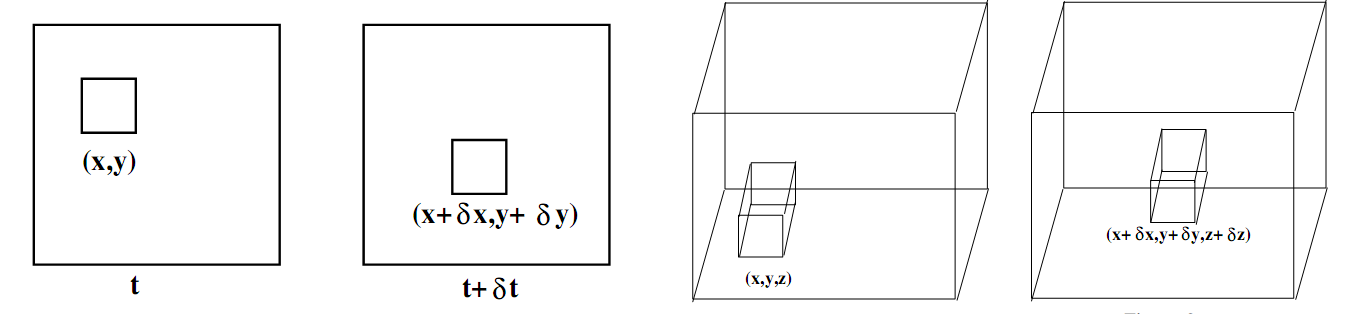
\includegraphics[scale = 0.3]{figures/2D_3D.png}} 
%  }
%  \caption[2D_3D]{Extension of optical flow methods for 3D. \textbf{Left:} Image model for 2D.  \textbf{Right:} Image model for 3D.}
%  \label{fig:2d_3d}
%\end{figure*}

The 2D variational \opticalflow model using the flow-driven smoothness approach (Section \ref{flow_driven}) is given by:
$$ E_{2D}(u,v) = \int_{\Omega_{2}}{(I(x+u,y+v,t+1) - I(x,y,t))^2 + \alpha \Psi(|\nabla_{2}u|^2 + |\nabla_{2}v|^2) \text{d}x \text{d}y}. $$
For a volume image $I(x,y,z,t)$, where $(x,y,z)$ are the voxel coordinates within an image domain $ \Omega_{3} \subset \mathbf{R}^3$, the extension to the 3D variational model reads:
\begin{eqnarray}
E_{3D}(u,v,w) &=& \int_{\Omega_{3}}{}(I(x+u,y+v, z+w, t+1) - I(x,y,z,t))^2 + \nonumber \\  
 &+& \alpha \: \Psi(|\nabla_{3}u|^2 + |\nabla_{3}v|^2 + |\nabla_{3}w|^2) \text{d}x \text{d}y \text{d}z. \nonumber
\end{eqnarray}

It is important to mention that some of the problems of 2D optical flow estimation disappear after the extension into a 3D domain. For example, there are no problems related to the projection geometry, such as occlusions between moving objects or divergent motion due to the perspective change.

As a drawback, solving 3D optical flow problem is a resources demanding task. It requires both large memory consumption and intense computational power. We further discuss performance aspects in Chapter \ref{performance} we describe a number of efficient computation schemes and present high-performance implementation of 3D optical flow methods on GPUs. 

\todo{Put examples of 3D data terms}  


%--------------------------------------------------------
\section{Numerical Solution}
%--------------------------------------------------------

In this section we explain how a variational optical flow model can be solved numerically. For this purpose we introduce a minimization procedure and iterative methods. We also discuss important implementation aspects, such as discretization and a derivatives approximation. In the first part of the section we derive underlying equations assuming small displacements between image frames.  Then we present an extension of the energy functional and its minimization procedure which allows to handle large displacements. To shorten the derivation of the corresponding formulas we assume 2D images. The extension to 3D domain can be performed in similar manner.   


\subsection{Minimization Procedure}
\label{minimization_procedure}

In the previous chapter we have discussed the construction of a variational energy functional. Next, our aim is to  find such a displacement field $u(x,y)$ and $v(x,y)$ which minimizes deviations from the model assumptions.

According to calculus of variations \cite{elsgolts62}, the minimum of the convex variational functional of the general form:
$$ E(u,v) = \int_{\Omega_{2}}{F(x,y,u, v, u_x, u_y, v_x, v_y})\text{d}x \text{d}y. $$
can be found at the location where its first-order derivatives vanish.
Such coupled differential equations are called \textit{Euler-Lagrange equations} and given by:
\begin{eqnarray}
F_u - \frac{\partial}{\partial x}F_{u_x} - \frac{\partial}{\partial y}F_{u_y} &=& 0 \\  \nonumber 
F_v - \frac{\partial}{\partial x}F_{v_x} - \frac{\partial}{\partial y}F_{v_y} &=& 0 
\label{eq:euler}	
\end{eqnarray}
with reflecting Neumann boundary conditions $\textbf{n}^\top \nabla u = 0$ and $\textbf{n}^\top \nabla v = 0$, where $\textbf{n}$ is a normal vector.


We show an example of minimization procedure on a flow-driven optical flow model with brightness constancy assumption. First, we calculate partial derivatives with respect to the unknown functions $u$ and $v$:
$$ F_u = 2 I^2_x u + 2 I_x I_y v + 2 I_x I_t $$ 
$$ F_v = 2 I_y I_x u + 2 I^2_y v + 2 I_y I_t $$
$$ F_{u_x} = 2 \alpha \: \Psi'(|\nabla u|^2 + |\nabla v|^2) \: u_x$$ 
$$ F_{u_y} = 2 \alpha \: \Psi'(|\nabla u|^2 + |\nabla v|^2) \: u_y$$
Embedding these terms into the Euler-Lagrange equations (\ref{eq:euler}) we obtain:
$$ I^2_x u + I_x I_y v + I_x I_t - \alpha \: \textrm{div} (\Psi'(|\nabla u|^2 + |\nabla v|^2) \cdot \nabla u ) = 0, $$
$$ I_y I_x u + I^2_y v + I_y I_t - \alpha \: \textrm{div} (\Psi'(|\nabla u|^2 + |\nabla v|^2) \cdot \nabla v ) = 0. $$
Solving this coupled system of equations with respect to the unknown displacement functions $u$ and $v$ gives us the minimum of our energy functional. 

\subsection{Discretization}
\label{discretization}

To solve Euler-Lagrange equations numerically we should perform a discretization procedure. We consider the unknown functions $u(x,y,t)$ and $v(x,y,t)$ on a rectangular image with the grid size of $h_x$ in $x$-direction and $h_y$ in $y$-direction. The values $u_{ij}$ and $v_{ij}$ denote the approximation of functions $u(x,y)$ and $v(x,y)$ at a pixel position $(i,j)$ with $i = 0 \ldots N-1, j=0 \ldots M-1$, where $N$, $M$ indicate image dimensions. 

In order to represent image derivatives we must assume a particular approximation of the differential operator. 
Second order approximations of the spatial image derivatives using central differences are given by:
$$ \left[ I_x \right]_{i,j} = \frac{I_{i+1,j,t} - I_{i-1,j,t} }{2 h_x} $$
$$ \left[ I_y \right]_{i,j} = \frac{I_{i,j+1,t} - I_{i,j-1,t} }{2 h_y} $$

To improve the accuracy of derivatives approximation one may also use fourth order approximations:
$$ \left[ I_x \right]_{i,j} = \frac{-I_{i+2,j,t} +  8  I_{i+1,j,t} - 8 I_{i-1,j,t} + I_{i-2,j,t} }{12 h_x} $$
$$ \left[ I_y \right]_{i,j} = \frac{-I_{i,j+2,t} +  8  I_{i,j+1,t} - 8 I_{i,j-1,t} + I_{i,j-2,t} }{12 h_y} $$

For further improvement with respect to noise it is common to use a temporal averaging of spatial derivatives \cite{Sun10, HarmonyFlow}.
For the second order central difference such a temporal averaging is given by:
$$ \left[ I_x \right]_{i,j} = \frac{(I_{i+1,j,t+1} - I_{i-1,j,t+1}) + (I_{i+1,j,t} - I_{i-1,j,t})  }{4 h_x} $$
$$ \left[ I_y \right]_{i,j} = \frac{(I_{i,j+1,t+1} - I_{i,j-1,t+1}) + (I_{i,j+1,t} - I_{i,j-1,t}) }{4 h_y} $$


To compute temporal derivatives we choose a forward difference:
$$ \left[ I_t \right]_{i,j} = \frac{I_{i,j,t+1} - I_{i,j,t}}{h_t},$$
where time step $h_t$ is chosen to be equal to 1.0.

We proceed with the discretization of others terms such as  $\textrm{div}(\Psi'(|\nabla u|^2 + |\nabla v|^2) \nabla u)$. 
Additionally to the second-order derivative approximation, we can also employ the discretization approach based on nested central differences with the halved grid sizes  $\frac{1}{2}h_x$ and $\frac{1}{2}h_y$.
Using this strategy the term $\textrm{div}(\Psi'\nabla u)$ can be expressed as: 
\begin{eqnarray}
\textrm{div}(\Psi'\nabla u) &=& (\Psi' u_x)_x + (\Psi' u_y)_y \nonumber \\
&=& \frac{ (\Psi' u_x)_{i + \frac{1}{2},j} - (\Psi' u_x)_{i - \frac{1}{2},j} }{2 (\frac{1}{2} h_x)} + 
\frac{ (\Psi' u_y)_{i,j + \frac{1}{2}} - (\Psi' u_y)_{i,j- \frac{1}{2}} }{2 (\frac{1}{2} h_y)} \nonumber \\
&=& \frac{\frac{\Psi'_{i+1,j} + \Psi'_{i,j}}{2} \left ( \frac{u_{i+1,j} - u_{i,j} }{2 (\frac{1}{2} h_x)} \right )   - \frac{\Psi'_{i,j} + \Psi'_{i-1,j}}{2}  \left (\frac{u_{i,j} - u_{i-1,j}}{2 (\frac{1}{2} h_x)} \right ) }  {2 (\frac{1}{2} h_x)} \nonumber \\
&+& \frac{\frac{\Psi'_{i,j+1} + \Psi'_{i,j}}{2} \left (  \frac{u_{i,j+1} - u_{i,j}}{2 (\frac{1}{2} h_y)} \right ) - \frac{\Psi'_{i,j} + \Psi'_{i,j-1}}{2} \left ( \frac{u_{i,j} - u_{i,j-1}}{2 (\frac{1}{2} h_y)} \right ) } {2 (\frac{1}{2} h_y)} \nonumber \\
 &=& \frac{\Psi'_{i+1,j} + \Psi'_{i,j}}{2} \left( \frac{u_{i+1,j} - u_{i,j}}{h^2_x} \right ) - \frac{\Psi'_{i,j} + \Psi'_{i-1,j}}{2} \left ( \frac{u_{i,j} - u_{i-1,j}}{h^2_x} \right ) \nonumber \\
 &+& \frac{\Psi'_{i,j+1} + \Psi'_{i,j}}{2} \left( \frac{u_{i,j+1} - u_{i,j}}{h^2_y} \right ) - \frac{\Psi'_{i,j} + \Psi'_{i,j-1}}{2} \left ( \frac{u_{i,j} - u_{i,j-1}}{h^2_y} \right ), \nonumber
\end{eqnarray}
where the nonlinear terms $[\Psi']_{i,j}$ are given by:
$$ [\Psi']_{i,j} = \Psi'(|\nabla u|^2 + |\nabla v|^2) = \Psi'([u_x]^2_{i,j} + [u_y]^2_{i,j} + [v_x]^2_{i,j} + [v_y]^2_{i,j}) $$ 
The discretization of  the term $\textrm{div}(\Psi'\nabla v)$ is done in a similar way.

Finally, after all necessary discretization schemes are introduced we can write down the discrete Euler - Lagrange equations:
$$ [I^2_x]_{i,j} u_{i,j} + [I_x I_y]_{i,j} v_{i,j} + [I_x I_t]_{i,j} - \alpha \: \sum_{l \in x,y} \sum_{(\bar{i}, \bar{j}) \in N_d(i,j)} \frac{[\Psi']_{\bar{i}, \bar{j}} + [\Psi']_{i,j} }{2} \Bigl (\frac{u_{\bar{i}, \bar{j}} - u_{i,j}  } {h^2_d} \Bigr) = 0 $$
$$ [I_y I_x]_{i,j} u_{i,j} + [I^2_y]_{i,j} v_{i,j} + [I_y I_t]_{i,j} - \alpha \: \sum_{l \in x,y} \sum_{(\bar{i}, \bar{j}) \in N_d(i,j)} \frac{[\Psi']_{\bar{i}, \bar{j}} + [\Psi']_{i,j} }{2} \Bigl (\frac{v_{\bar{i}, \bar{j}} - v_{i,j}  } {h^2_d} \Bigr) = 0, $$
where $N_d(i,j)$ denotes neighbor pixels for the position $(i,j)$ in the direction $d \in (x,y)$.

Now, this coupled system of equations has to be solved with respect to the unknown displacements $u_{ij},  v_{ij}$. 

\subsection{Iterative Methods}
\label{iterative_methods}

After the discretization of the Euler-Lagrange equations is performed we obtain a linear system of equations, which can be formulated in the following form:
$$ A \textbf{x} = \textbf{b} $$
To solve it directly, we may invert the system matrix and multiply it by the result vector:
$$ \textbf{x} = A^{-1} \textbf{b} $$
However, for large systems of equations this procedure is computationally expensive. As an alternative, it is possible to decompose the initial matrix $A$ into two terms:
$$ A = A_1 + A_2, $$
and try to approximate the solution iteratively: 
$$ A_1 \textbf{x}^{k+1} = \textbf{b} - A_2 \textbf{x}^k $$
$$ \textbf{x}^{k+1} = A_1^{-1} (\textbf{b} - A_2 \textbf{x}^k)$$
The appropriate choice of matrix $A^{-1}_1$ should be done in such a way, that it is a good approximation to the initial inverse matrix $A^{-1}$. Additionally, it should be easily computable. This matrix splitting strategy is a core idea for a number of iterative methods such as \textit{Jacobi} and \textit{Gau\ss - Seidel methods}. 

\subsubsection{Jacobi method}
\label{jacobi_method}



The Jacobi method is an iterative algorithm to solve a system of linear equations \cite{Saad03}. The system of linear equations $A \textbf{x} = \textbf{b}$ has an unique solution, if the coefficient matrix $A$ contains no zeros on its main diagonal. On each iteration step, one finds the approximate solution for each diagonal element and use it in the next step. The iterative process is then repeated until it converges. 

The Jacobi method can be expressed in a matrix form, using the following decomposition of the initial matrix $A$:
%
\begin{equation}
A = D - L - U,
\end{equation}
%
where $D$, $L$ and $U$ represent the diagonal, strictly lower triangular and strictly upper triangular matrices of $A$, respectively. After the substitution of the decomposed matrix $A$ in the equation $A \textbf{x} = \textbf{b}$, it can be reformulated in the following way::
%
\begin{equation}
D \textbf{x} = (L + U)\textbf{x} + \textbf{b},
\end{equation}
%
and the corresponding iterative solution can be found via:
%
\begin{equation}
\textbf{x}^{k+1} = D^{-1}(L + U)\textbf{x}^{k} + D^{-1}\textbf{b}.
\end{equation}


Using the Jacobi method, the new value of $x_i^{k}$ on the iteration step $k+1$ can be estimated in the following way:
%
\begin{equation}
x_i^{k+1} = \frac{1}{a_{ii}} \left( 
b_i - 
\sum_{j=1, j \neq i}^{n} \left( a_{ij}x_j^{k}
\right) \right) .
\end{equation}

It is important to mention that  the order in which the matrix entries are evaluated is irrelevant since the Jacobi method uses only the matrix values from the old time step. Such property of the method is advantageous for the parallel implementations of the iterative algorithm.




\subsubsection{The Gau\ss -Seidel Method}
\label{gauss_method}

One of the most simple and commonly used iterative solvers for linear system of equations is the Gau\ss -Seidel method \cite{Saad03}. In this approach the initial matrix A is decomposed into the following parts:
$$ A = D - L - U = \underbrace{(D - L)}_{A_1} + \underbrace{(-U)}_{A_2}, $$
where $D, L, U$ represent the diagonal, strictly lower triangular, and strictly upper triangular parts of the system matrix $A$. Using such decomposition we can rewrite the initial equations:
$$ (D-L)\textbf{x} = (\textbf{b}+ U \textbf{x}) $$
The solution using  Gau\ss -Seidel methods is then given by:
$$ \textbf{x} = (D-L)^{-1}(\textbf{b}+ U \textbf{x}). $$
And the corresponding iterative solution scheme reads:
$$ \textbf{x}^{k+1} = (D-L)^{-1}(\textbf{b}+ U \textbf{x}^{k}). $$






\subsection{Large Displacements}
\label{large_displacements}

In Section \ref{discretization} we assumed that displacements between two consequent images are  small, so the linearization of the data constancy assumption can be performed. This procedure is important since it allows us to construct convex energy functionals, which we can minimize using globally convergent algorithms. However, in case of a large displacements the linearization procedure cannot be performed, since no reliable approximation is possible using the Taylor expansion. In order to handle whole range of displacements in this section we introduce an extension of the variational approach and describe the steps related to its minimization.

\subsubsection{Euler - Lagrange Equations}

As a first step, we formulate the energy functional in its original form  without linearized data constraints:
\begin{eqnarray}
E(u,v) = \int_{\Omega_{2}} {(I(x+u, y+v, t+1) - I(x, y, t))^2 + \alpha \Psi(|\nabla_{2}u|^2 + |\nabla_{2}v|^2) dx dy}.
\label{eq:energy_func}	
\end{eqnarray}
The corresponding Euler-Lagrange equations, which have to be solved to find the minimum of the energy functional are given by:
$$ I_{x}(x+u, y+v, t+1) (I(x+u, y+v, t+1) - I(x, y, t)) - \alpha \: \textrm{div} (\Psi'(|\nabla u|^2 + |\nabla v|^2) \cdot \nabla u ) = 0,   $$
$$ I_{y}(x+u, y+v, t+1) (I(x+u, y+v, t+1) - I(x, y, t)) - \alpha \: \textrm{div} (\Psi'(|\nabla u|^2 + |\nabla v|^2) \cdot \nabla v ) = 0   $$

Note, that the energy functional (\ref{eq:energy_func}) is not convex, since the data term implicitly depends on the unknown flow components $u, v$. From the non-convexity property it follows that multiple local minima may exist and numerical algorithms could be trapped in such a local minimum away from the best solution.

In order to find a solution the incorporation of a suitable minimization strategy is required.


\subsubsection{Coarse-to-fine Strategy}
\label{coarse_strategy}

The common approach to deal with large displacements in many optical flow methods is a coarse-to-fine strategy \cite{Black96, Memin98, Brox04}. In the current work we follow this idea and use the incremental hierarchical approach. First, on each computation level we decompose the flow field into an already computed solution from the previous coarser level $u,v$ and a small unknown motion increment for the current level $du,dv$ (see Figure \ref{fig:coarse_to_fine}):
$$ u^{k+1} = u^{k} + du^{k}, $$
$$ v^{k+1} = v^{k} + dv^{k}. $$
\begin{figure*}[h]
  \centerline{
    \mbox{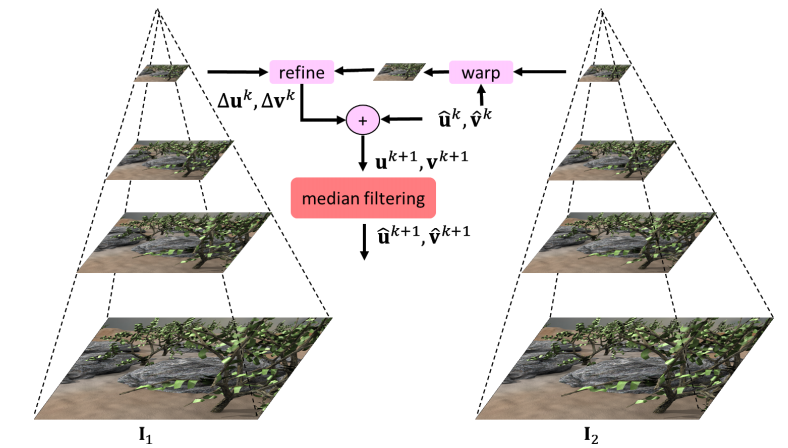
\includegraphics[scale = 0.45]{figures/coarse_to_fine.png}} 
  }
  \caption[coarse_to_fine]{A schematic example of a multi-level coarse-to-fine computation strategy. The top level of image pyramids represent the coarsest level and the bottom level of pyramid corresponds to the original image representation. The computation scheme includes image warping \ref{compensation} and median filtering of intermediate flow results \ref{flow_median}.  Image: \cite{Sun14}}
  \label{fig:coarse_to_fine}
\end{figure*}

Putting the incremental definition of the overall flow field we rewrite the image function $I(x+u^{k+1}, y+v^{k+1}, t+1)$ in the following way:
$$ I(x+u^{k+1}, y+v^{k+1}, t+1) = I(x+u^{k}+du^{k}, y+v^{k}+dv^{k}, t+1) $$
Next, we perform a first-order Taylor expansion around the point $I(x+u^{k+1}, y+v^{k+1}, t+1)$, which gives us:
\begin{eqnarray}
I(x+u^{k}+du^{k}, y+v^{k}+dv^{k}, t+1) &=& I(x+u^{k}, y+v^{k}, t+1) \nonumber \\ &+& I_{x}(x+u^{k}, y+v^{k}, t+1)du^{k} \nonumber \\ &+& I_{y}(x+u^{k}, y+v^{k}, t+1)dv^{k} \nonumber
\end{eqnarray}
Finally we can write the Euler-Lagrange equations:
\begin{eqnarray}
I_{x}(x+u^k, y+v^k, t+1) (& & I_{x}(x+u^{k}, y+v^{k}, t+1)du^{k} \nonumber \\ &+&  I_{y}(x+u^{k}, y+v^{k}, t+1)dv^{k} \nonumber \\ &+& I(x+u^{k}, y+v^{k}, t+1) - I(x,y,t)) \nonumber \\ &-& \alpha \: \textrm{div} (\Psi'(|\nabla (u^{k} + du^{k})|^2 + |\nabla (v^{k} + dv^{k} )|^2) \cdot \nabla (u^{k} + du^{k}) ) = 0 \nonumber
\end{eqnarray}
\begin{eqnarray}
I_{y}(x+u^k, y+v^k, t+1) (& & I_{x}(x+u^{k}, y+v^{k}, t+1)du^{k} \nonumber \\ &+&  I_{y}(x+u^{k}, y+v^{k}, t+1)dv^{k} \nonumber \\ &+& I(x+u^{k}, y+v^{k}, t+1) - I(x,y,t)) \nonumber \\ &-& \alpha \: \textrm{div} (\Psi'(|\nabla (u^{k} + du^{k})|^2 + |\nabla (v^{k} + dv^{k} )|^2) \cdot \nabla (v^{k} + dv^{k}) ) = 0 \nonumber
\end{eqnarray}

This system of equations has to be solved on each computation level $k$ with respect to the motion increments $du^{k}$ and $dv^{k}$. Since we assume that these increments are small the linearization procedure is valid and can be applied. After the flow increments for the current level are computed we find the overall solution as $u^{k+1} = u^{k} + du^{k}, v^{k+1} = v^{k} + dv^{k}$. With such a coarse-to-fine strategy we perform the flow computation step-by-step, so instead of a non-convex optimization we solve a series of convex problems and successively refine the result.
 
In order to implement such a hierarchical approach we have to consider an appropriate implementation to obtain the motion compensated image $I(x+u^k, y+v^k, t+1)$ at a computation level $k$  and the realization of a multi-level strategy (construction of image pyramids).

%----------------- TO CHECK ------------------

%\change{From: \cite{Secrets}. We adaptively determine the number of pyramid levels so that the top level has a width or height of around 20 to 30 pixels.}
%\comment{Give small discussion here}
%\change{From: \cite{Middl}. A limitation of many coarse-to-fine algorithms, however, is the tendency to over-smooth fine structure and to fail to capture small fast-moving objects. Make a reference to Middl paper}


\subsubsection{Motion Compensation}
\label{compensation}

We first discuss the implementation of the motion compensation procedure. The computation of the image function $I(x+u, y+v, t+1)$ and its derivatives $I_x(x+u, y+v, t+1)$, $I_y(x+u, y+v, t+1)$ requires to "apply"  the computed flow field on the initial image, so-called \textit{image warping} \cite{Memin98}.  In this work we follow the approach proposed in \cite{Memin98, Brox04} and perform a \textit{backward registration}. A number of different implementations are possible (see Section \ref{multilevel}). Here we show an example of motion compensation using bilinear interpolation.

We decompose the real-valued computed flow field $u$ and $v$ into two parts: $u = \hat{u}  + \epsilon_u, v = \hat{v}  + \epsilon_v$ where $\hat{u}, \hat{v}$ denote the integer fraction of $u, v$ and $\epsilon_u, \epsilon_v$ denote the subpixel displacement. Then we compute the motion compensated image $I(x+u,y+v,t+1)$ by means of bilinear interpolation using:
\begin{eqnarray*}
[I(x+u,y+v,t+1)]_{i,j,t+1} = & & (1-\epsilon_u)(1 - \epsilon_v) I_{(i+\hat{u}),(j+\hat{v}), t+1} \\
&+& ( \epsilon_u)(1 - \epsilon_v) I_{(i+\hat{u}) + 1,(j+\hat{v}), t+1} \\
&+& (1-\epsilon_u)(\epsilon_v) I_{(i+\hat{u}),(j+\hat{v})+1, t+1}  \\
&+& (\epsilon_u)(\epsilon_v) I_{(i+\hat{u})+1,(j+\hat{v})+1, t+1} 
\end{eqnarray*}
The motion compensation procedure for the image derivatives $I_x(x+u,y+v,t+1)$, $I_y(x+u,y+v,t+1)$ can be performed in the analogous way.

\subsection{Multi-level Computation}
\label{multilevel}

In order to implement a coarse-to-fine strategy we need to specify a transfer function which downscales the original image version to a coarser resolution level and interpolates the obtained results back to the finer computation level. 
On each computation level $k$ the image size is determined via:
$$ N^k_{d} = N^{orig} _{d} \eta^k,$$
where $\eta$ is a warping scale parameter, $N_d$ denotes the image size in the dimension $d \in (x,y)$.

For this purpose a number of approaches can be used such as nearest neighbour averaging, area-based averaging \cite{Bruhn05}, billinear or bicubic interpolation. 
%-------------------------------
%  Not useful
%-------------------------------
%\begin{figure*}[ht]
%  \centerline{
%    \mbox{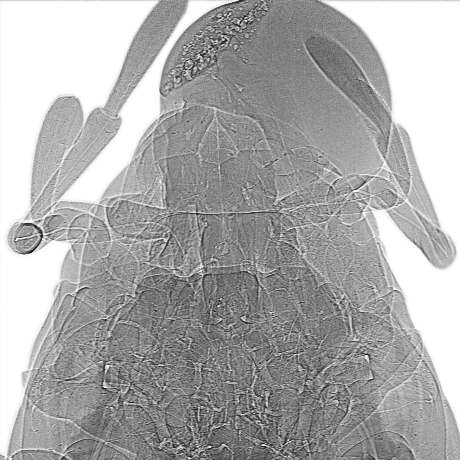
\includegraphics[scale=0.3]{figures/bug_scale1.png}}
%    \mbox{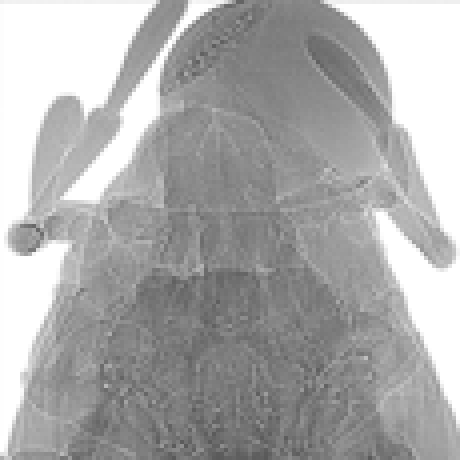
\includegraphics[scale=0.3]{figures/bug_scale4.png}}
%    \mbox{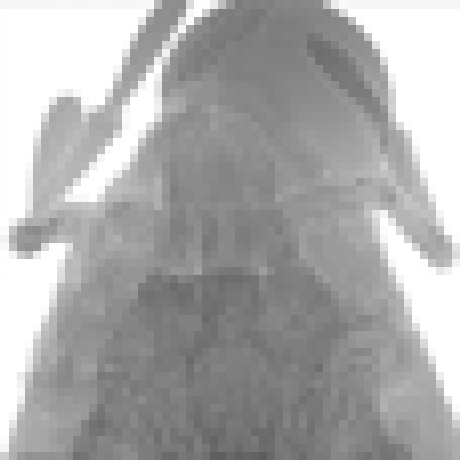
\includegraphics[scale=0.3]{figures/bug_scale8.png}}
%  }
%  \caption[]{Image pyramid constructed using bicubic interpolation on different computation levels. \textbf{Left:} Original level. Original size = (460, 460). \textbf{Center:} Coarse scale = 0.25. Coarse size = (115, 115). \textbf{Right:} Coarse scale = 0.125. Coarse size = (57, 57).}
%  \label{fig:image_pyramid}
%\end{figure*}
In the current work for the construction of image pyramids we use bicubic interpolation using Coons patches \cite{Coons67}. This method gives good results \cite{Sun14, HarmonyFlow}, efficient and easy to implement. For the case of using 3D tomographic data as an input, we employ tricubic interpolation.



\subsection{Intermediate Flow Filtering}
\label{flow_median}

In the work of \cite{Sun10, Sun14} authors reveal a preprocessing step which allows to significantly improve the accuracy and, which  is more important, robustness of optical flow estimation \cite{Wedel09}. It is proposed to apply a median filtering to the intermediate flow result prior to the warping step to the next computation level.

The reason for its surprisingly good results is straightforward. The errors in flow estimation which appear on the coarse image scale are propagated via a warping step to the next level. On this level the incorrect flow serves as an initialization for optical flow estimation.  This results in an accumulation of errors during incremental computation procedure. The median filtering allows to suppress flow errors already on earlier computation levels. With this approach the current optical flow solution is computed via $\textbf{w}^{k+1} = M_p (\textbf{w}^{k} +\textbf{dw}^{k})$, where $M$ is a median filter and $p$ is its mask size. 

In \cite{Sun10, Sun14} it is concluded that optimal size of the median mask is ($5 \times 5$), which outperforms both ($3 \times 3$) and ($7 \times 7$) settings.
In our work we generalize the median filtering approach and use a more adaptive strategy for the flow correction. First, we might observe that on the most coarse computation level, when the image size is the smallest (around 20-50 pixels) median mask of size ($5 \times 5$) may oversmooth the flow result, which can lead to inaccurate flow estimation. To avoid that, we apply less strict filtering on coarse levels using a smaller mask of $3 \times 3$ pixels.

Additionally, in the presence of high amounts of noise or severe artifacts we use a selective filtering using a larger mask ($7 \times 7$ and $9 \times 9$ ). We perform such filtering in homogeneous image regions determined using the same median filtering ($7 \times 7$ or $9 \times 9$) on the original image.  
We present evaluation results in the experimental section \ref{exp_flow_median}.

% \subsection{Anti-aliasing}
% \label{antialiasing}

% In the recent work of \cite{HarmonyFlow} it was shown that high frequency brightness variations in combination with certain amount of displacements can introduce artifacts related to image aliasing.
% The authors proposed to apply a low-pass filtering prior to downsampling for the construction of image pyramids.

% Since X-ray data can potentially contain such high frequency features (for example, morphological structures, tissues, etc) we follow the idea presented in \cite{Sun14} and apply Gaussian filter with a standard deviation $ \frac{1}{\sqrt{2 \eta}} $, where $\eta$ denotes the downsampling factor.


%\subsection{[OPTIONAL] Data Range}
%
%\begin{itemize}
%	\item Discuss the influence of extended data bit range on precision of OF.
%	\item Show on examples: 8-bit and 32-bit floating point \comment{How to make a GT image for floating point?}
%\end{itemize}



%%--------------------------------------------------------
%\section {Performance}
%\label{performance}
%%--------------------------------------------------------
%
%\subsection{Motivation}
%
%\subsection{Advanced Numerical Schemes}
%\label{advanced_numerics}
%
%\subsubsection{Successive-Overrelaxation}
%
%\comment{Write down possible disadvantages. Oversmoothing?}
%
%\subsubsection{Adaptive Interations}
%
%Adapt number of iterations according to current warping level: the less is the size -- the less iteratins we need. Show difference 
%
%\subsubsection{Multigrid Methods}
%
%\comment{What else? Should be added something}
%
%%\section{Input splitting strategies}
%%Including multiprocessors and GRID
%
%\subsection{Efficient Strategies}
%\label{efficient_strategies}
%
%
%\subsubsection{Efficient multi-level strategy}
%\todo{Add more information about efficient implementation of multi-level strategy. \cite{CGF3013}}
%\change{From: \cite{CGF3013} Adaptive multi-scale strategy which tries to isolate image regions where the flow changes slowly. In these regions we replace the computationally expensive energy minimization operation by a simple interpolation. } 
%
%
%\subsubsection{Combining Different Algorithms}
%
%\todo{Give reference to Fusion Flow paper}
%\comment{Add information about combination of efficient and fast implementation with a successive run of high precision OF implementation . From \cite{CGF3013} Show references}
%
%\subsection{Parallelization on  GPU}   
%\label{gpu} 
%
%\todo{Check and include references}
%\change{From: \cite{HarmonyFlow} Following the trend of parallel
%implementations on modern GPUs (Zach et al. 2007;
%Grossauer and Thoman 2008; Sundaram et al. 2010; Werlberger
%et al. 2010) we recently came up with a GPU version
%of our method that can compute flow fields of size 640×480
%pixels in less than one second (Gwosdek et al. 2010).}
%


%--------------------------------------------------------
\section{Summary}
%--------------------------------------------------------

In this section we summarize all models and features which are available in our optical flow framework. In  Table \ref{tab:models_overview} we provide the references to the original papers, where a particular approach  was introduced or discussed, as well as give a reference to the corresponding parts of this work. 
\renewcommand{\arraystretch}{1.2}
\begin{table}[!ht]  \small
  \centering
  \caption{A summary of methods implemented within the optical flow framework presented in this work.}
\begin{tabular}{ |l|l|l|l| } 
%\begin{tabular}{ |c|c|p{7cm}|c| }
\hline
 & Model & References & Section \\ \hline
\multirow{8}{*}{\begin{sideways} Data term \hspace{0pt} \end{sideways}}
 & Brightness constancy 	& \cite{LucasKanade81, HornSchunck81} & \ref{brightness_constancy_assumption}  \\
 & Gradient constancy 	& \cite{Schnorr93, Brox04, Papenberg06} 	& \ref{gradient} \\
 & Higher-order derivatives & \cite{Papenberg06} 							& \ref{high_order_constancy} \\
 & Multiple image features & \cite{Brox04, HarmonyFlow} 				& \ref{assumptions_on_multiple_image_features} \\
 & Combined Local-Global& \cite{Bruhn02, Bruhn05a} 						& \ref{clg} \\
 & Robust Modeling & \cite{Black91, Black96, Sun14, Middl} 			& \ref{robust} \\
 & Joint and Separate Modeling & \cite{Bruhn05b, HarmonyFlow}		& \ref{joint_and_separate} \\
 & Data Normalization & \cite{Lai98, HarmonyFlow} 						& \ref{normalization} \\ 
\hline
\multirow{5}{*}{\begin{sideways}Smoothness \hspace{3pt}\end{sideways}} 
 & Homogeneous & \cite{HornSchunck81}   &  \ref{homogeneous_smoothness} \\
 & Image-driven & \cite{Schnorr93, Alvarez99, Weickert00b}   & \ref{image_driven}  \\
 & Flow-driven &  \cite{Schnorr94, Brox04, Papenberg06}   & \ref{flow_driven}  \\
 & Spatial-temporal & \cite{Nagel90, Weickert2001b}    & \ref{spatial_temporal} \\
 & Adaptive smoothness & \cite{HarmonyFlow}   & \ref{adaptive_smoothness} \\ 
\hline
\multirow{6}{*}{\begin{sideways}Optimisation\end{sideways}} 
 & Coarse-to-fine strategy & \cite{Black96, Memin98, Brox04}   & \ref{coarse_strategy} \\
 & Flow median filtering & \cite{Wedel09, Sun14}   & \ref{flow_median} \\
 %& Anti-aliasing & \cite{HarmonyFlow, Sun14}   & \ref{antialiasing} \\
 & Multiple results fusion & \cite{Lempitsky08}   & \ref{assumptions_on_multiple_image_features} \\
 & User-driven landmarks & \cite{Fischer03}     & \ref{landmarks} \\
 & Confidence measures & \cite{Fua93, Brown03, Bruhn06, Xu10}   & \ref{confidence_measures} \\
 & Parameters optimization & \cite{HarmonyFlow}   & \ref{parameters_optimization} \\ 
\hline
\multirow{3}{*}{\begin{sideways} Compute \hspace{7pt}  \end{sideways}} 
 & 2D images & ---    &  \ref{data_constancy_assumptions}, \ref{smoothness_assumptions} \\
 & 3D images & ---    &  \ref{extension_3d} \\
 & Efficient schemes & \cite{Brox04, BruhnThesis, CGF3013}    &  \ref{advanced_numerics}  \\
 & GPU computation & ---   & \ref{gpu} \\
\hline
\end{tabular}
\label{tab:models_overview}
\end{table}
